\chapter{Boundary Value Problems}
\section{Systems of equations}
An m-th order system of equation of first order \addtoindex{Initial Value Problem} can be expressed in the form
\begin{equation}\label{sys eqn}
\begin{array}{cl}
\frac{du_1}{dt}=f_1(t,u_1,...,u_m) \\ 
\frac{du_2}{dt}=f_2(t,u_1,...,u_m) \\ 
.\\
.\\
.\\
\frac{du_m}{dt}=f_m(t,u_1,...,u_m) 
\end{array}
\end{equation}
for $a \leq t \leq b$ with the the initial conditions
\begin{equation}\label{sys con}
\begin{array}{cl}
u_1(a)=\alpha_1\\
u_2(a)=\alpha_2\\
.\\
.\\
.\\
u_m(a)=\alpha_m.
\end{array}
\end{equation}
This can also be written in vector from
\[\mathbf{u^{'}}=\mathbf{f}(t,\mathbf{u}) \]
with initial conditions
\[\mathbf{u(a)=\alpha}.
\]
\begin{definition}
The function $f(t,u_1,...,u_m)$ defined on the set
\[
D=\{(t,u_1,..,u_m)|a\leq t \leq b, -\infty < u_i < \infty, i=1,..,m \}
\]
is said to be a \textbf{\addtoindex{Lipschitz Condition}} on D in the variables $u_1,...,u_m$ if a
constant $L$, the Lipschitz Constant, exists with the property that 
\[ |f(t,u_1,...,u_m)-f(t,z_1,z_2,...,z_m)| \leq L \sum_{j=1}^{m}|u_j-z_j| \]
for all $(t,u_1,...,u_m)$ and $(t,z_1,z_2,...,z_m)$ in $D$.
\end{definition}
\begin{theorem}
Suppose
\[
D=\{(t,u_1,..,u_m)|a\leq t \leq b, -\infty < u_i < \infty, i=1,..,m \}
\]
is continuous on $D$ and satisfy a \addtoindex{Lipschitz Condition}.  The system of 1st order
equations subject th the initial conditions, has a unique solution
$u_1(t),u_2(t),...,u_m(t)$ for $a\leq t \leq b$.
\end{theorem}
\begin{example}
Using Euler method on the system\[
\begin{array}{cl}
u'=u^2-2uv \ \ \ u(0)=1\\
v'=tu+u^2sinv \ \ \ v(0)=-1
\end{array}
\]
for $0\leq t \leq 0.5$ and $h=0.05$
the general Euler difference system of equations is of the form
\[\begin{array}{cl}
\hat{u}_{i+1}=\hat{u}_{i}+hf(t_i,\hat{u}_i,\hat{v}_i) \\
\hat{v}_{i+1}=\hat{v}_{i}+hg(t_i,\hat{u}_i,\hat{v}_i) 
\end{array}
\]
Applied the the \addtoindex{Initial Value Problem}
\[\begin{array}{cl}
\hat{u}_{i+1}=\hat{u}_{i}+0.05(\hat{u}_i^2-2\hat{u}_i\hat{v}_i) \\
\hat{v}_{i+1}=\hat{v}_{i}+0.05(t_i\hat{u}_i+\hat{u}_i^2sin(\hat{v}_i)) 
\end{array}
\]
We know for $i=0$, $\hat{u}_0=1$ and $\hat{v}_0=-1$ from the initial
conditions.\\
For i=0 we have
\[\begin{array}{cl}
\hat{u}_{1}=\hat{u}_{0}+0.05(\hat{u}_0^2-2\hat{u}_0\hat{v}_0) =1.15\\
\hat{v}_{1}=\hat{v}_{0}+0.05(t_0\hat{u}_0+\hat{u}_0^2sin(\hat{v}_0))=-1.042 
\end{array}
\]
and so forth.
\end{example}
\section{Higher order Equations}
\begin{definition}
A general mth order initial value problem
\[y^{(m)}(t)=f(t,y,...,y^{(m-1)}) \ \ a\leq t \leq b \]
with initial conditions
\[y(a)=\alpha_1, y^{'}(a)=\alpha_2,...,y^{(m-1)}(a)=\alpha_m \]
can be converted into a system of equations as in (\ref{sys eqn}) and (\ref{sys con})\\
Let $u_1(t)=y(t), u_1(t)=y^{1}(t),...,u_m(t)=y^{(m-1)}(t) $. This produces
the first order system of equations

\[
\begin{array}{cl}
\frac{du_1}{dt}=\frac{dy}{dt}=u_2\\
\frac{du_2}{dt}=\frac{dy^{'}}{dt}=u_3\\
.\\
.\\
.\\
\frac{du_{m-1}}{dt}=\frac{dy^{(m-2)}}{dt}=u_m\\
\frac{du_m}{dt}=\frac{dy^{(m-1)}}{dt}f_m(t,y,...,y^{(m-1)})=f(t,u_1,...,u_m)
\end{array}
\]
with initial conditions
\[
\begin{array}{cl}
u_{1}(a)=y(a)=\alpha_1\\
u_{2}(a)=y^{'}(a)=\alpha_2\\
.\\
.\\
.\\
u_{m}(a)=y^{(m-1)}(a)=\alpha_m\\
\end{array}
\]
\end{definition}
\begin{example}
\[ y^{''}+3y^{'}+2y=e^t\]
with initial conditions $y(0)=1$ and $y^{'}(0)=2$ can be converted to the system
\[
\begin{array}{cl}
u^{'}=v &u(0)=1\\
v^{'}=e^t-2u-3v &v(0)=2
\end{array}
\]
the difference Euler equation is of the form
\[
\begin{array}{cl}
\hat{u}_{i+1}=\hat{u}_i+hv(t_i,\hat{u}_i,\hat{v}_i)\\
\hat{v}_{i+1}=\hat{v}_i+h(e^{t_i}-2\hat{u}_i-3\hat{v}_i)\\
\end{array}
\]
\end{example}
\section{Boundary Value Problems}
Consider the second order differential equation
\begin{equation}
\label{2nd order ODE}
y^{''}=f(x,y,y^{'})
\end{equation}
defined on an interval $a \leq x \leq b$.  Here $f$ is a function of three variables and $y$ is an unknown.  The general solution to \ref{2nd order ODE}
contains two arbitrary constants so in order to determine it uniquely it is necessary to impose two additional conditions on $y$.  When one of these is given at $x=a$
and the other at $x=b$ the problem is called a 
\addtoindex{boundary value problem} and associated conditions are called boundary conditions.\\
The simplest type of boundary conditions are
\[y(a)=\alpha\]
\[y(b)=\beta \]
for a given numbers $\alpha$ and $\beta$.  However more general conditions such as
\[\lambda_1 y(a)+\lambda_2 y^{'}(a)=\alpha_1 \]
\[\mu_1 y(b)+\mu_2 y^{'}(b)=\alpha_2 \]
for given numbers $\alpha_i, \lambda_i$ and $\mu_i$ (i=1,2) are sometimes imposed.\\
Unlike \addtoindex{Initial Value Problem} whose problems are uniquely solvable \addtoindex{boundary value problem} can have no solution or many.
\begin{example}
The differential equation
\[ y^{''}+y=0\]
\[y_1(x)=y(x) \ \ \ y_2(x)=y^{'}(x)\]
\[y^{'}_1=y_2 \]
\[y^{'}_2=-y_1 \]
It has the general solution 
\[w(x) = C_1sin(x)+C_2 cos(x)\]
where $C_1,C_2$ are constants.\\
The special solution $w(x)=sin(x)$ is the only solution that satisfies 
\[ w(0)=0 \ \ \ w(\frac{\pi}{2})=1 \]
All functions of the form $w(x)=C_1sin(x)$ where $C_1$ is an arbitrary constant,
satisfies
\[ w(0)=0 \ \ \ w(\pi)=0 \]
while there is no solution for the boundary conditions
\[ w(0)=0 \ \ \ w(\pi)=1. \]
 $\diamond$
\end{example}
While we cannot state that all \addtoindex{boundary value problem} are unique we can say a few things.
\section{Some theorems about {boundary value problem}}
Writing the general linear subset \addtoindex{Boundary Value Problem}
\begin{equation}\label{linear BVP}
\begin{array}{l}
y^{''}=p(x)y^{'}+q(x)y+g(x) \ \ \ a < x < b \\
A\left(\begin{array}{c} y(a) \\ y^{'}(a) \end{array} \right)
+
B\left(\begin{array}{c} y(b) \\ y^{'}(b) \end{array} \right)
=
\left(\begin{array}{c} \gamma_1 \\ \gamma_2 \end{array} \right)
\end{array}
\end{equation}
The homogeneous problem is the case in which $g(x)$ and $\gamma_1=\gamma_2=0$.
\begin{theorem}
The non-homogeneous problem (\ref{linear BVP}) has a unique solution $y(x)$ on 
$[a,b]$ for each set of given $\{g(x),\gamma_1,\gamma_2 \}$ if and only if the 
homogeneous problem has only the trivial solutions $y(x)=0$.
\end{theorem}
For conditions under which the homogeneous problem (\ref{linear BVP}) has only
the zero solution we consider the following subset of problem
\begin{equation}\label{linear subset BVP}
\begin{array}{l}
y^{''}=p(x)y^{'}+q(x)y+g(x) \ \ \ a < x < b \\
a_0 y(a)-a_1  y^{'}(a) =\gamma_1 \\
 b_0y(b) +b_1 y^{'}(b) = \gamma_2 \\
\end{array}
\end{equation}
Assume the following conditions
\begin{equation}
\begin{array}{ll}
q(x)>0 & a\leq x \leq b \\
a_0,a_1 \geq 0 & b_0,b_1 \geq 0 \\
\end{array}
\end{equation}
$|a_1|+|a_0|\not= 0, |b_1|+|b_0|\not= 0,|a_0|+|b_0|\not= 0$
Then the homogeneous problem for (\ref{linear subset BVP}) has only the zero solution
therefore the theorem is applicable and the non-homogeneous problem has a unique
solution for each set of data $\{g(x),\gamma_1,\gamma_2 \}$.\\
The theory for a non-linear problem is far more complicated than that of a linear problem. Looking at the class of problems
\begin{equation}\label{non-linear BVP}
\begin{array}{l}
y^{''}=f(x,y,y^{'}) \ \ \ a < x < b \\
a_0 y(a)-a_1  y^{'}(a) =\gamma_1 \\
 b_0y(b) +b_1 y^{'}(b) = \gamma_2 \\
\end{array}
\end{equation}
The function $f$ is assumed to satisfy the following \addtoindex{Lipschitz Condition}
\begin{equation}\label{non-linear Lipschitz BVP}
\begin{array}{l}
|f(x,u_1,v_1)-f(x,u_2,v_2)| \leq K_1|u_1-u_2|\\
|f(x,u_1,v_1)-f(x,u_2,v_2)| \leq K_2|v_1-v_2|\\
\end{array}
\end{equation}
for all points in the region
\[ R=\{(x,u,v)| a\leq x \leq b, -\infty < u,v < \infty \}\]
\begin{theorem}
The problem (\ref{non-linear BVP}) assumes $f(x,u,v)$ is continuous on the region
$R$ and it satisfies the \addtoindex{Lipschitz condition} (\ref{non-linear Lipschitz  BVP}).  In
addition assume that $f$, on $R$, satisfies
\[\frac{\partial f(x,u,v)}{\partial u}> 0 \ \ \ \left|\frac{\partial f(x,u,v)}{\partial v} \right|\leq M \]
for some constant $M>0$ for the boundary conditions of \ref{non-linear BVP} assume
that $|a_1|+|a_0|\not= 0, |b_1|+|b_0|\not= 0,|a_0|+|b_0|\not= 0$.
The \addtoindex{boundary value problem} has a unique solution.
\end{theorem}
\begin{example}
The boundary value problem \addtoindex{boundary value problem}
\[ y^{''} +e^{-xy}+sin(y^{'})=0 \ \ \ 1 < x < 2\]
with $y(1)=y(2)=0$, has
\[ f(x,y,y^{'})=-e^{-xy}-sin(y^{'})\]
Since 
\[\frac{\partial f(x,y,y^{'})}{\partial y} =xe^{xy} >0 \]
and
\[\left|\frac{\partial f(x,y,y^{'})}{\partial y^{'}}\right| =|-cos(y^{'}) \leq1 \]
this problem has a unique solution.
$\diamond$
\end{example}
\section{Shooting Methods}
The principal of the shooting method is to change our original boundary value problem \addtoindex{boundary value problem} into 2 \addtoindex{Initial Value Problem}.
\subsection{Linear Shooting method}
Looking at problem class (\ref{linear subset BVP}).  We break this down into two
\addtoindex{Initial Value Problem}.
\begin{equation}
\begin{split}
 y^{''}_1=p(x)y^{'}_1+q(x)y_1+r(x), \ \    y_1(a)=\alpha, \ \ y^{'}_1(a)=0\\
y^{''}_2=p(x)y^{'}_2+q(x)y_2, \ \ y_2(a)=0, \ \ y^{'}_2(a)=1
\end{split}
\end{equation}


combining these results together to get the unique solution 
\begin{equation}
y(x)=y_1(x)+\frac{\beta-y_1(b)}{y_2(b)}y_2(x)
\end{equation}
provided that $y_2(b)\not=0$.
\begin{example}
\[ y^{''}=2y^{'}+3y-6 \]
with boundary conditions
\[y(0) = 3 \]
\[y(1) = e^3+2 \]
The exact solution is 
\[y=e^{3x}+2 \]
breaking this \addtoindex{boundary value problem} into two \addtoindex{Initial Value Problem}'s
\begin{equation}
\label{Shoot A}
y^{''}_1 =2y^{'}_1+3y_{1}-6 \ \ \ \ y_1(a)=3, \ \ \ y^{'}_1(a)=0\end{equation}
\begin{equation}
\label{Shoot B}
y^{''}_2 =2y^{'}_2+3y_{2} \ \ \ \ y_2(a)=0, \ \ \ y^{'}_2(a)=1\end{equation}
Discretising (\ref{Shoot A})
\[ y_1=u_1 \ \ \ y_1^{'}=u_2\]
\[u_1^{'}=u_2 \ \  u_1(a)=3\]
\[u_2^{'}=2u_2+3u_1-6 \ \ \ u_2(a)=0\]
using the Euler method we have the two difference equations
\[u_{1 i+1}=u_{1 i} + h u_{2 i}\]
\[u_{2 i+1}=u_{2 i} + h (2u_{2 i}+3u_{1 i} -6)\]
Discretising (\ref{Shoot B})
\[ y_2=w_1 \ \ \ \  y_2^{'}=w_2\]
\[w_1^{'}=w_2 \ \ \  w_1(a)=0\]
\[w_2^{'}=2w_2+3w_1 \ \ \ w_2(a)=1\]
using the Euler method we have the two difference equations
\[w_{1 i+1}=w_{1 i} + h w_{2 i}\]
\[w_{2 i+1}=w_{2 i} + h (2w_{2 i}+3w_{1 i})\]
combining all these to get our solution
\[y_i=u_{1 i} + \frac{\beta-u_{1}(b)}{w_1(b)}w_{1 i}\]
It can be said 
\[ |y_i - y(x_i)| \leq K h^n\left|1+\frac{w_{1 i}}{u_{1 i}}\right| \]
$O(h^n)$ is the order of the method.
\end{example}


\begin{figure}[H]
\centering
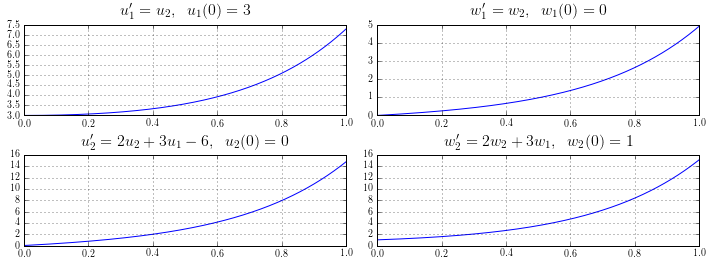
\includegraphics[scale=0.5]{Shooting_linear_method_all}
\caption{Python output: Shooting Method}
\label{Shooting_method}
\end{figure}

\begin{figure}[H]
\centering
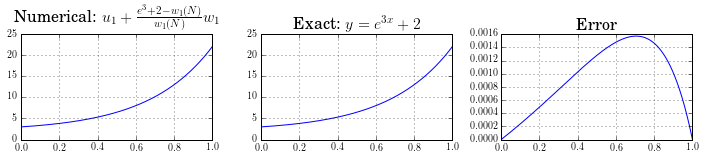
\includegraphics[scale=0.5]{Shooting_linear_method_Num_analyt_error}
\caption{Python output: Shooting Method error}
\label{Shooting_method_error}
\end{figure}

\subsection{The Shooting method for non-linear equations}
\begin{example}
\[y^{''}=-2yy^{'} \ \ \ y(0)=0 \ \ y(1)=1\]
The corresponding initial value problem is 
\begin{equation}\label{shoot non-lin}
y^{''}=-2yy^{'} \ \ \ y(0)=0 \ \  y^{'}(0)=\lambda \end{equation}
Which reduces to the first order system, letting $y_1=y$ and $y_2=y^{'}$. 
\[ y^{'}_1=y_2 \ \ \ y_1(0)=0 \]
\[y^{'}_2=-2y_1y_2 \ \ \ y^{'}_2(0)=\lambda \]
Taking $\lambda =1$ and $\lambda=2$ as the first and second guess of $y^{'}(0)$.
(\ref{shoot non-lin}) depends on two variable $x$ and $\lambda$.
$\diamond$
\end{example}
\textbf{How to choose $\lambda$?}\\
Our goal is to choose $\lambda$ such that.
\[F(\lambda)=y(b,\lambda)-\beta=0 \]
We use \addtoindex{Newton's method} to generate the sequence $\lambda_k$ with only the initial approx $\lambda_0$.
The iteration has the form
\[\lambda_k=\lambda_{k-1}-\frac{y(b,\lambda_{k-1})-\beta}{\frac{dy}{d \lambda}(b,\lambda_{k-1})}\]
and requires knowledge of $\frac{dy}{d \lambda}(b,\lambda_{k-1})$.  This present
a difficulty since an explicit representation for $y(b,\lambda)$ is unknown we only know
$y(b,\lambda_0),$ $y(b,\lambda_1),...,y(b,\lambda_{k-1})$.\\
Rewriting our \addtoindex{Initial Value Problem} we have it so that it depends on both $x$ and $\lambda$.
\[ y^{''}(x,\lambda)=f(x,y(x,\lambda),y^{'}(x,\lambda)) \ \ a\leq x \leq b\]
\[y(a,\lambda)=\alpha \ \ y^{'}(a,\lambda)=\lambda \]
differentiating with respect to $\lambda$ and let $z(x,\lambda)$ denote $\frac{\partial y}{\partial\lambda}(x,\lambda)$ we have
\[
\frac{\partial }{\partial \lambda}(y^{''}) = \frac{\partial f}{\partial \lambda}=\frac{\partial f}{\partial y}
\frac{\partial y}{\partial \lambda}+
\frac{\partial f}{\partial y^{'}}
\frac{\partial y^{'}}{\partial \lambda}
\]
Now 
\[\frac{\partial y^{'} }{\partial \lambda}=\frac{\partial}{\partial \lambda}\frac{\partial y}{\partial x}
=\frac{\partial }{\partial x}\left( \frac{\partial y}{\partial \lambda}\right)
=\frac{\partial z}{\partial x}=z^{'}\]
we have
\[ z^{''}(x,\lambda)=\frac{\partial f}{\partial y}z(x,\lambda)+\frac{\partial f}{\partial y^{'}}z^{'}(x,\lambda) \]
for $a \leq x \leq b$ and the boundary conditions
\[z(a,\lambda)=0, \ \ \ z^{'}(a,\lambda)=1 \]
Now we have 
\[\lambda_k=\lambda_{k-1}-\frac{y(b,\lambda_{k-1})-\beta}{z(b,\lambda_{k-1})}\]
We can solve the original non-linear subset \addtoindex{Boundary Value Problem} by solving the 2 \addtoindex{Initial Value Problem}'s.
\begin{example}(cont.)\\
\[\frac{\partial f}{\partial y}=-2y^{'} \ \ \ \frac{\partial f}{\partial y^{'}}=-2y\]
We now have the two \addtoindex{Initial Value Problem}'s
\[y^{''}=-2yy^{'} \ \ \ y(0)=0 \ \ y^{'}(0)=\lambda \]
\begin{eqnarray*}
z^{''}&=&\frac{\partial f}{\partial y}z(x,\lambda)+\frac{\partial f}{\partial y^{'}}z^{'}(x,\lambda)\\
&=&-2y^{'}z-2yz^{'} \ \ z(0)=0 \ \ z^{'}(0)=1 \end{eqnarray*}
Discretising we let $y_1=y$, $y_2=y^{'}$, $y_3=z$ and $y_4=z^{'}$.
\begin{eqnarray*}
y_1^{'}=y_2 &\ \ : \ \  &y_1(0)=0 \\
y_2^{'}=-2y_1y_2 &\ \ : \ \  &y_2(0)=\lambda_k \\
z_1^{'}=z_2 &\ \ : \ \  &z_1(0)=0 \\
z_2^{'}=-2z_1y_2-2y_1z_2 &\ \ : \ \  &y_2(0)=1 
\end{eqnarray*}
with
\[\lambda_k=\lambda_{k-1}-\frac{y_1(b)-\beta}{y_3(b)} \]
Then solve using a one step method.
$\diamond$
\end{example}


\begin{figure}[H]
\centering
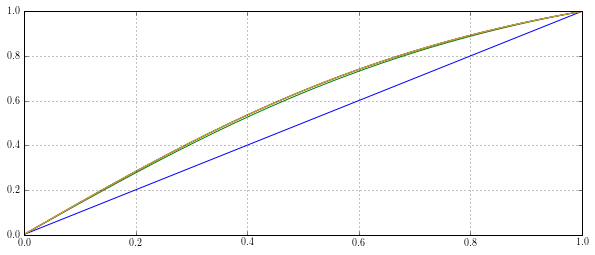
\includegraphics[scale=0.5]{Shooting_nonlinear_method_all}
\caption{Python output: Nonlinear Shooting Method}
\label{Shooting_method_nl}
\end{figure}

\begin{figure}[H]
\centering
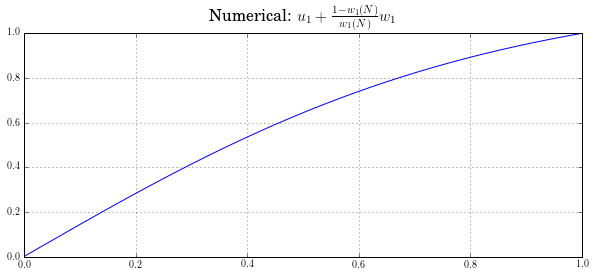
\includegraphics[scale=0.5]{Shooting_nonlinear_method_solnl}
\caption{Python output: Nonlinear Shooting Method result}
\label{Shooting_method_error}
\end{figure}

\begin{figure}[H]
\centering
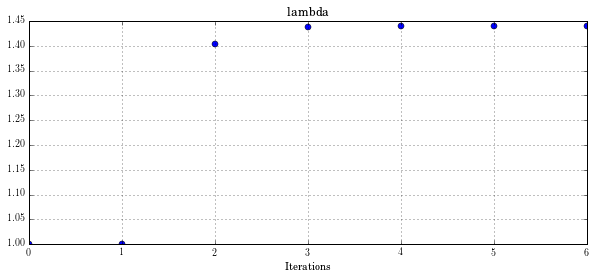
\includegraphics[scale=0.5]{Shooting_nonlinear_method_lambda}
\caption{Python output: Nonlinear Shooting Method $\lambda$}
\label{Shooting_method_error}
\end{figure}



\section{Finite Difference method}
Each finite difference operator can be derived from Taylor expansion.\\
Once again looking at a linear second order differential equation
\[y^{''}=p(x)y^{'}+q(x)y+r(x) \]
on $[a,b]$ subject to boundary conditions
\[ y(a)=\alpha \ \ \ y(b) =\beta \]
As with all cases we divide the area into even spaced mesh points
\[x_0=a, \ \ x_N=b \ \ \ x_i=x_0+ih \ \ h=\frac{b-a}{N} \]
We now replace the derivatives $y^{'}(x)$ and $y^{''}(x)$ with the centered difference approximations
\[y^{'}(x)=\frac{1}{2h}(y(x_{i+1})-y(x_{i-1}))-\frac{h^2}{12}y^{3}(\xi_i) \]
\[y^{''}(x)=\frac{1}{h^2}(y(x_{i+1})-2y(x_i)+y(x_{i-1}))-\frac{h^2}{6}y^{4}(\mu_i) \]
for some $x_{i-1} \leq \xi_i \mu_i \leq x_{i+1}$ for i=1,...,N-1.\\
We now have the equation
\[
\frac{1}{h^2}(y(x_{i+1})-2y(x_i)+y(x_{i-1}))=p(x_i)\frac{1}{2h}(y(x_{i+1})-y(x_{i-1}))+q(x_i)y(x_i)+r(x_i)\]
This is rearranged such that we have all the unknown together,
\[\left(1+\frac{hp(x_i)}{2} \right)y(x_{i-1})-(2+h^2q(x_i))y(x_i)+\left(1-\frac{hp(x_i)}{2} \right)y(x_{i+1})=h^2r(x_i) \]
for $i=1,..,N-1$.\\
Since the values of $p(x_i),q(x_i)$ and $r(x_i)$ are known it represents a linear
algebraic equation involving $y(x_{i-1}), y(x_{i}),y(x_{i+1})$.\\
This produces a system of $N-1$ linear equations with $N-1$ unknowns $y(x_1),...,y(x_{N-1})$.\\
The first equation corresponding to $i=1$ simplifies to 
\[-(2+h^2q(x_1))y(x_1)+\left(1-\frac{hp(x_1)}{2} \right)y(x_{2})=h^2r(x_1)-\left(1+\frac{hp(x_1)}{2} \right)\alpha \]
because of the boundary condition $y(a)=\alpha$, and for $i=N-1$
\[ \left(1+\frac{hp(x_{N-1})}{2} \right)y(x_{N-2}) -(2+h^2q(x_{N-1}))y(x_{N-1})=h^2r(x_{N-1})-\left(1-\frac{hp(x_{N-1})}{2} \right)\beta \]
because $y(b)=\beta$.\\
The values of $y_i, \ (i=1,...,N-1)$ can therefore be found by solving the tridiagonal system
\[A\mathbf{y}=\mathbf{b} \]
where
\[
A =\]
\[\begin{bmatrix}
-(2+h^2q(x_1)) & \left(1-\frac{hp(x_1)}{2}\right) & 0 &.&0 \\
 \left(1+\frac{hp(x_2)}{2}\right)&-(2+h^2q(x_2)) & \left(1-\frac{hp(x_2)}{2}\right) & 0 &.  \\
0&.&.&0&0\\
.&.&.&.&.\\
.&.&.&.&.\\
 .&0&\left(1+\frac{hp(x_{N-2})}{2}\right)&-(2+h^2q(x_{N-2})) & \left(1-\frac{hp(x_{N-2})}{2}\right) \\
 .&0&0&\left(1+\frac{hp(x_{N-1})}{2}\right)&-(2+h^2q(x_{N-1})) 
\end{bmatrix}
\]
\[
y =\left( \begin{array}{c}
y_1 \\
y_2 \\
. \\
. \\
y_{N-2} \\
y_{N-1} 
\end{array}\right)
b =\left( \begin{array}{c}
h^2r_1-\left( 1+\frac{hp_1}{2}\right)\alpha \\
h^2r_2 \\
. \\
. \\
h^2r_{N-2} \\
h^2r_{N-1}-\left( 1-\frac{hp_1}{2}\right)\beta
\end{array}\right)
\]
\begin{example}
Looking at the simple case
\[\frac{d^2y}{dx^2}=4y, \ \ y(0)=1.1752, \ \ y(1)=10.0179. \]
Our difference equation is
\[
\frac{1}{h^2}(y(x_{i+1})-2y(x_i)+y(x_{i-1}))=4y(x_i) \ \ \ i=1,..,N-1 \]
dividing $[0,1]$ into 4 subintervals we have $h=\frac{1-0}{4}$
\[x_i=x_0+ih=0+i(0.25)\]
In this simple example $q(x)=4$, $p(x)=0$ and $r(x)=0$. Rearranging the
equation we have
\[ \frac{1}{h^2} (y(x_{i+1})) -\left(\frac{2}{h^2}+4\right)y(x_i) +\frac{1}{h^2} (y(x_{i-1}))=0\]
multiplying across by $h^2$
\[  y(x_{i+1}) -(2+4h^2)y(x_i) + (y(x_{i-1}))=0\]
with the boundary conditions $y(x_0)=1.1752$ and $y(x_4)=10.0179$.
Our equations are of the form
\begin{eqnarray*}
y(x_2)-2.25y(x_1)=-1.1752\\
y(x_3)-2.25y(x_2)+y(x_1)=0\\
-2.25y(x_3)+y(x_2)=-10.0179
\end{eqnarray*}
Putting this into matrix form 
\[\left(\begin{array}{ccc} -2.25&1&0\\
1&-2.25&1\\
0&1&-2.25
\end{array}\right)
\left(\begin{array}{c} y_1\\
y_2\\
y_3
\end{array}\right)
=
\left(\begin{array}{c}-1.1752\\
0\\
-10.0179 \end{array}\right)
\]
\begin{center}
\begin{tabular}{l|l|c}
$x$ & $y$ & Exact $sinh(2x+1)$\\
\hline
0 & 1.1752&1.1752\\
0.25 & 2.1467 & 2.1293\\
0.5 & 3.6549& 3.6269\\
0.75 & 6.0768& 6.0502\\
1.0& 10.0179& 10.0179\\
\end{tabular}
\end{center}
\end{example}$\diamond$
\begin{example}
Looking at a more involved \addtoindex{boundary value problem}
\[y^{''}=xy^{'}-3y+e^x \ \ \ y(0)=1 \ \ y(1)=2 \]
Let N=5 then $h=\frac{1-0}{5}=0.2$. The difference equation is of the form
\[
\frac{1}{h^2}(y(x_{i+1})-2y(x_i)+y(x_{i-1}))=x_i\frac{1}{2h}(y(x_{i+1})-y(x_{i-1}))-3y(x_i)+e^{x_i}\]
Re arranging and putting $h=0.2$
\[(1+\frac{0.2(x_i)}{2})y(x_{i-1})-(1.88)y(x_i)+(1-\frac{0.2(x_i)}{2})y(x_{i+1})=0.04e^{x_i} \]
In matrix form this is
\[\left(\begin{array}{cccc} -1.88&0.98&0&0\\
1.04&-1.88&0.96&0\\
0&1.06&-1.88&0.94\\
0&0&1.08&-1.88
\end{array}\right)
\left(\begin{array}{c} y_1\\
y_2\\
y_3\\
y_4
\end{array}\right)
=
\left(\begin{array}{c}
0.04e^{0.2}-1.02\\
0.04e^{0.4}\\
0.04e^{0.6}\\
0.04e^{0.8}-1.84 
\end{array}\right)
\]
$y_1=1.4651$, $y_2=1.8196$, $y_3=2.0283$ and $y_4=2.1023$.
\end{example}
\section*{Solving a tri-diagonal system}
To solve a tri-diagonal system we can use the method discussed in the approximation theory.

